\documentclass{article}

\usepackage{graphicx}
\usepackage{subfigure}
\usepackage{booktabs}
\usepackage{hyperref}

% Attempt to make hyperref and algorithmic work together better:
\newcommand{\theHalgorithm}{\arabic{algorithm}}

% Use the following line for the initial blind version submitted for review:
% \usepackage{icml2021}

% If accepted, instead use the following line for the camera-ready submission:
\usepackage[accepted]{icml2021}

% The \icmltitle you define below is probably too long as a header.
% Therefore, a short form for the running title is supplied here:
\icmltitlerunning{Sparse Self-Attention GCNs for Improved Learning Runtime}

\begin{document}

\twocolumn[
\icmltitle{
  PROPOSAL: 
  Sparse Self-Attention in Graph Convolutional Networks \\
  for Improved Structure Learning Runtime
}

% It is OKAY to include author information, even for blind
% submissions: the style file will automatically remove it for you
% unless you've provided the [accepted] option to the icml2021
% package.

% List of affiliations: The first argument should be a (short)
% identifier you will use later to specify author affiliations
% Academic affiliations should list Department, University, City, Region, Country
% Industry affiliations should list Company, City, Region, Country

% You can specify symbols, otherwise they are numbered in order.
% Ideally, you should not use this facility. Affiliations will be numbered
% in order of appearance and this is the preferred way.
\icmlsetsymbol{equal}{*}

\begin{icmlauthorlist}
\icmlauthor{Anton Chen}{equal,ubc}
\icmlauthor{Xiang Xi Chen}{equal,ubc}
\end{icmlauthorlist}

\icmlaffiliation{ubc}{Department of Computer Science, University of British Columbia, Vancouver, B.C., Canada}

\icmlcorrespondingauthor{Anton Chen}{contact@antonchen.ca}
\icmlcorrespondingauthor{Xiang Xi Chen}{xiangxi.chen.ca@gmail.com}

% You may provide any keywords that you
% find helpful for describing your paper; these are used to populate
% the "keywords" metadata in the PDF but will not be shown in the document
\icmlkeywords{Machine Learning, ICML}

\vskip 0.3in
]

% this must go after the closing bracket ] following \twocolumn[ ...

% The command takes one argument, which is text to display at the start of the footnote.
% The \icmlEqualContribution command is standard text for equal contribution.
% Remove it (just {}) if you do not need this facility.

%\printAffiliationsAndNotice{}  % leave blank if no need to mention equal contribution
\printAffiliationsAndNotice{\icmlEqualContribution} % otherwise use the standard text.

\begin{abstract}
  Graph Convolutional Networks (GCNs)
  are increasingly popular architectures for 
  representation learning and downstream tasks on
  graph-structured data.
  % Homophily is an important characteristic of graph data
  % which describes how ``similar'' nearby nodes are to each other.
  While the majority of modern GCNs face difficulty 
  learning low-homophily graphs,
  a recent approach (GCN-SA) 
  successfully captures long-range dependencies
  using multi-head self-attention.
  However GCN-SA is self-admittedly limited by the poor
  runtime scaling of its self-attention mechanism.
  We propose the use of sparse self-attention mechanisms
  (e.g. Big Bird, Performer) to replace GCN-SA's attention
  mechanisms to
  reduce SA runtime from quadratic to linear.
  As noted in the mentioned sparse SA literature,
  we expect minimal performance degradation
  while improving GCN-SA's runtime.
\end{abstract}

\section{Context and Problem}
\label{submission}

\subsection{Graph-Structured Data and GCNs}

It's no secret that
many real-world problems involve graph-structured data,
including classification on social networks,
academic paper citations,
webpage links,
and so on.
Graph Convolutional Networks (GCNs)
have evolved as generalizations of CNNs,
and are considered the most promising
architecture to handle graph data,
having already been used successfully in numerous
applications \cite{hamilton2017representation}.

\subsection{Non-Homophilous Graphs Pose Problems}

One glaring issue that modern GCNs face is the task
of learning low-homophily graphs \cite{fan2023markov}.

Homophily in graph data refers to the tendency for nodes with
similar features to be closely connected \cite{li2023homogcl}.
For instance,
in a professional network,
people tend to be connected with similar individuals
(e.g. similar industry, position, years of experience, etc.), 
illustrating an example of a high-homophily graph.
An example of a low-homophily graph is a subway system
where stations serve as a hub for diverse individuals 
with varying demographics, interests, and use for the subway.

Modern GCNs tend to perform poorly on low-homophily graph data,
including Geom-GCN \cite{pei2020geom}
and H\textsubscript{2}GCN \cite{zhu2020beyond}.
This is due to such approaches relying on
feature representations that only consider
adjacent neighbor nodes,
failing to capture long-range correlations \cite{jiang2024self}.
Jiang et al. takes this into account in their
newly proposed model. 

\subsection{GCN-SA, Full Self-Attention, and Poor Runtime}

Jiang et al. (March 2024) introduces GCN-SA,
an architecture which leverages multi-head self-attention
(MHSA) to effectively learn node and edge embeddings
in both low and high-homophily graphs \cite{jiang2024self}.

What sparks our interest the most about GCN-SA
is its creative use of a self-attention mechanism:
MHSA is used to learn a new adjacency matrix
where self-attention identifies highly-correlated nodes,
and transforms the adjacency matrix such that they become neighbors.
In particular, long-distance correlations can be uncovered,
resulting in better performance on low-homophily datasets.

A significant limitation of GCN-SA mentioned by \cite{jiang2024self} 
is the poor runtime complexity
caused by its full self-attention mechanism,
which necessitates $ n^2 $ pairwise operations
for $ n $ nodes.
Our main motivation for this project is to reduce the
``excessive computational burden'', which becomes particularly
problematic when dealing with incredibly large non-homophilous graphs 
in practice \cite{lim2021large}.

\subsection{Sparse Self Attention: Big Bird, Performers, etc.}

Outside of graph learning,
researchers have found great success in
efficient long-range attention
with the rise of sparse self-attention mechanisms
\cite{
  zaheer2020big, 
  choromanski2020rethinking, 
  beltagy2020longformer}.
Rather than computing all pairwise similarity scores,
sparse self-attention mechanisms
compute a small subset of similarity scores,
yielding a sparse score matrix in a fraction of the time.
In fact, self-attention runtime complexity is reduced from 
\textit{quadratic} runtime to \textit{linear} runtime.

The fact that the resulting score matrix is sparse is not an issue 
--- it is actually desired. 
A sparse score matrix corresponds to less edge connections
in the reconnected adjacency matrix.
Jiang et al. even intend to ensure the reconnected adjacency is sparse,
with a $ k $-NN and minimum-threshold approach to selecting attention.
Linear attention will do this all for us --- and faster.

Sparse attention methods such as Performers, a linear
attention framework that approximate the standard attention matrix
into lower-rank randomized matrices \cite{choromanski2020rethinking},
and Big Bird, a framework that does not require 
prerequisite knowledge about source data structures \cite{zaheer2020big},
have successfully acted as generic drop-in replacements
for full self-attention,
showing promise in new domains without
existing domain knowledge.
This motivates the use of such methods in GCN-SA
for graph learning.

\section{Proposed Plan, Procedure, and Experiments}

Our high-level idea is to 
modify GCN-SA's self-attention-based
adjacency matrix transforming mechanism
with various sparse self-attention mechanisms.
We'll focus on classification accuracy and 
runtime of the modified models
against baseline GCN-SA.

More specifically, our plan includes:
\begin{enumerate}
  \item Technical overview of GCN-SA's full self-attention mechanism,
    focusing on the mathematics.
  \item Technical overview of sparse (and linear) 
    self-attention mechanisms.
  \item Creating multiple variations of GCN-SA,
    each with linear self-attention layers 
    (e.g. one model with Big Bird layers, one model with Performer layers, etc.)
  \item Perform training/validation/testing on one of the 8 datasets,
    similar to Jiang et al.'s method.
    We'll also experiment with varying hyperparameters
    via cross-validation,
    e.g. number of heads in self-attention.
  \item Repeat on all 8 datasets of varying degrees of homophily,
  \item Introduce more linear self-attention mechanisms if time permits.
  \item Compare runtime and classification accuracy. 
    Draw conclusions, make reflections, etc.
\end{enumerate}

\subsection{Available Source Code and Datasets}

Source code for GCN-SA,
Big Bird, and Performers
is available on GitHub.
After some preliminary investigation into the codebases,
GCN-SA implements self-attention with in a
custom PyTorch module.
Big Bird and Performers expose linear self-attention 
as layers, so minimal ``model surgery'' is required.

We'll be using the 8 open graph datasets
used in Jiang et al.'s study.
Note that these datasets have varying degrees
of homophily,
so we are especially interested
in performance on the low-homophily datasets.

\subsection{Time Constraints}

To vary the scope of the project,
we may reduce the number of sparse self-attention techniques
used, or the number of datasets trained on.

\section{Potential Impact and Contribution}

We'd like to see significant runtime improvements
with similar performance for these sparse
self-attention models. If successful, we can greatly
reduce the time it takes to train large and
non-homophilous graphs. As mentioned previously, 
this has widespread applications
in social network data, global trade data, etc and
can make meaningful real world contributions.
Improved training runtime can open up the door
for possibilities including 
better downstream accuracy,
or the ability to use larger datasets.

% \begin{figure}[ht]
% \vskip 0.2in
% \begin{center}
% \centerline{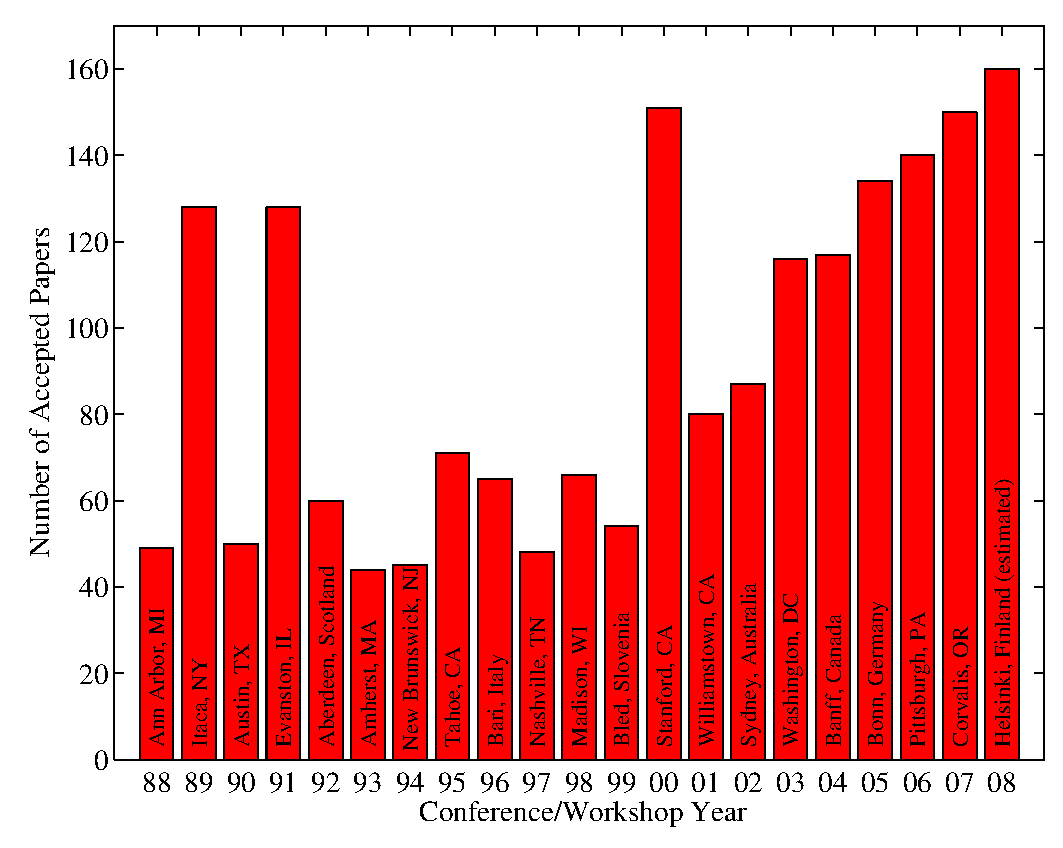
\includegraphics[width=\columnwidth]{icml_numpapers}}
% \caption{Historical locations and number of accepted papers for International
% Machine Learning Conferences (ICML 1993 -- ICML 2008) and International
% Workshops on Machine Learning (ML 1988 -- ML 1992). At the time this figure was
% produced, the number of accepted papers for ICML 2008 was unknown and instead
% estimated.}
% \label{icml-historical}
% \end{center}
% \vskip -0.2in
% \end{figure}

% \subsection{Figures}

% You may want to include figures in the paper to illustrate
% your approach and results. Such artwork should be centered,
% legible, and separated from the text. Lines should be dark and at
% least 0.5~points thick for purposes of reproduction, and text should
% not appear on a gray background.

% Label all distinct components of each figure. If the figure takes the
% form of a graph, then give a name for each axis and include a legend
% that briefly describes each curve. Do not include a title inside the
% figure; instead, the caption should serve this function.

% Number figures sequentially, placing the figure number and caption
% \emph{after} the graphics, with at least 0.1~inches of space before
% the caption and 0.1~inches after it, as in
% Figure~\ref{icml-historical}. The figure caption should be set in
% 9~point type and centered unless it runs two or more lines, in which
% case it should be flush left. You may float figures to the top or
% bottom of a column, and you may set wide figures across both columns
% (use the environment \texttt{figure*} in \LaTeX). Always place
% two-column figures at the top or bottom of the page.

% \subsection{Algorithms}

% If you are using \LaTeX, please use the ``algorithm'' and ``algorithmic''
% environments to format pseudocode. These require
% the corresponding stylefiles, algorithm.sty and
% algorithmic.sty, which are supplied with this package.
% Algorithm~\ref{alg:example} shows an example.

% \begin{algorithm}[tb]
%    \caption{Bubble Sort}
%    \label{alg:example}
% \begin{algorithmic}
%    \STATE {\bfseries Input:} data $x_i$, size $m$
%    \REPEAT
%    \STATE Initialize $noChange = true$.
%    \FOR{$i=1$ {\bfseries to} $m-1$}
%    \IF{$x_i > x_{i+1}$}
%    \STATE Swap $x_i$ and $x_{i+1}$
%    \STATE $noChange = false$
%    \ENDIF
%    \ENDFOR
%    \UNTIL{$noChange$ is $true$}
% \end{algorithmic}
% \end{algorithm}

% \subsection{Tables}

% You may also want to include tables that summarize material. Like
% figures, these should be centered, legible, and numbered consecutively.
% However, place the title \emph{above} the table with at least
% 0.1~inches of space before the title and the same after it, as in
% Table~\ref{sample-table}. The table title should be set in 9~point
% type and centered unless it runs two or more lines, in which case it
% should be flush left.

% % Note use of \abovespace and \belowspace to get reasonable spacing
% % above and below tabular lines.

% \begin{table}[t]
% \caption{Classification accuracies for naive Bayes and flexible
% Bayes on various data sets.}
% \label{sample-table}
% \vskip 0.15in
% \begin{center}
% \begin{small}
% \begin{sc}
% \begin{tabular}{lcccr}
% \toprule
% Data set & Naive & Flexible & Better? \\
% \midrule
% Breast    & 95.9$\pm$ 0.2& 96.7$\pm$ 0.2& $\surd$ \\
% Cleveland & 83.3$\pm$ 0.6& 80.0$\pm$ 0.6& $\times$\\
% Glass2    & 61.9$\pm$ 1.4& 83.8$\pm$ 0.7& $\surd$ \\
% Credit    & 74.8$\pm$ 0.5& 78.3$\pm$ 0.6&         \\
% Horse     & 73.3$\pm$ 0.9& 69.7$\pm$ 1.0& $\times$\\
% Meta      & 67.1$\pm$ 0.6& 76.5$\pm$ 0.5& $\surd$ \\
% Pima      & 75.1$\pm$ 0.6& 73.9$\pm$ 0.5&         \\
% Vehicle   & 44.9$\pm$ 0.6& 61.5$\pm$ 0.4& $\surd$ \\
% \bottomrule
% \end{tabular}
% \end{sc}
% \end{small}
% \end{center}
% \vskip -0.1in
% \end{table}

% Tables contain textual material, whereas figures contain graphical material.
% Specify the contents of each row and column in the table's topmost
% row. Again, you may float tables to a column's top or bottom, and set
% wide tables across both columns. Place two-column tables at the
% top or bottom of the page.

% \subsection{Citations and References}

% Please use APA reference format regardless of your formatter
% or word processor. If you rely on the \LaTeX\/ bibliographic
% facility, use \texttt{natbib.sty} and \texttt{icml2021.bst}
% included in the style-file package to obtain this format.

% Citations within the text should include the authors' last names and
% year. If the authors' names are included in the sentence, place only
% the year in parentheses, for example when referencing Arthur Samuel's
% pioneering work \yrcite{Samuel59}. Otherwise place the entire
% reference in parentheses with the authors and year separated by a
% comma \cite{Samuel59}. List multiple references separated by
% semicolons \cite{kearns89,Samuel59,mitchell80}. Use the `et~al.'
% construct only for citations with three or more authors or after
% listing all authors to a publication in an earlier reference \cite{MachineLearningI}.

% Authors should cite their own work in the third person
% in the initial version of their paper submitted for blind review.
% Please refer to Section~\ref{author info} for detailed instructions on how to
% cite your own papers.

% Use an unnumbered first-level section heading for the references, and use a
% hanging indent style, with the first line of the reference flush against the
% left margin and subsequent lines indented by 10 points. The references at the
% end of this document give examples for journal articles \cite{Samuel59},
% conference publications \cite{langley00}, book chapters \cite{Newell81}, books
% \cite{DudaHart2nd}, edited volumes \cite{MachineLearningI}, technical reports
% \cite{mitchell80}, and dissertations \cite{kearns89}.

% Alphabetize references by the surnames of the first authors, with
% single author entries preceding multiple author entries. Order
% references for the same authors by year of publication, with the
% earliest first. Make sure that each reference includes all relevant
% information (e.g., page numbers).

% Please put some effort into making references complete, presentable, and
% consistent. If using bibtex, please protect capital letters of names and
% abbreviations in titles, for example, use \{B\}ayesian or \{L\}ipschitz
% in your .bib file.

\bibliography{proposal}
\bibliographystyle{icml2021}


%%%%%%%%%%%%%%%%%%%%%%%%%%%%%%%%%%%%%%%%%%%%%%%%%%%%%%%%%%%%%%%%%%%%%%%%%%%%%%%%
%%%%%%%%%%%%%%%%%%%%%%%%%%%%%%%%%%%%%%%%%%%%%%%%%%%%%%%%%%%%%%%%%%%%%%%%%%%%%%%%
%% DELETE THIS PART. DO NOT PLACE CONTENT AFTER THE REFERENCES!
%%%%%%%%%%%%%%%%%%%%%%%%%%%%%%%%%%%%%%%%%%%%%%%%%%%%%%%%%%%%%%%%%%%%%%%%%%%%%%%%
%%%%%%%%%%%%%%%%%%%%%%%%%%%%%%%%%%%%%%%%%%%%%%%%%%%%%%%%%%%%%%%%%%%%%%%%%%%%%%%%
%\appendix
%\section{Do \emph{not} have an appendix here}

%\textbf{\emph{Do not put content after the references.}}
%%
%Put anything that you might normally include after the references in a separate
%supplementary file.

%We recommend that you build supplementary material in a separate document.
%If you must create one PDF and cut it up, please be careful to use a tool that
%doesn't alter the margins, and that doesn't aggressively rewrite the PDF file.
%pdftk usually works fine. 

%\textbf{Please do not use Apple's preview to cut off supplementary material.} In
%previous years it has altered margins, and created headaches at the camera-ready
%stage. 
%%%%%%%%%%%%%%%%%%%%%%%%%%%%%%%%%%%%%%%%%%%%%%%%%%%%%%%%%%%%%%%%%%%%%%%%%%%%%%%%
%%%%%%%%%%%%%%%%%%%%%%%%%%%%%%%%%%%%%%%%%%%%%%%%%%%%%%%%%%%%%%%%%%%%%%%%%%%%%%%%


\end{document}
